%%=====================================================================
%%  2 微信小程序开发介绍
%%=====================================================================
\section{微信小程序开发介绍}

\subsection{微信小程序系统架构}

微信小程序采用了视图层与逻辑层分离的双线程架构，其结构层次如图 \ref{fig:architecture} 所示\cite{bib:lei}。

\begin{figure}[htbp]
  \centering
  \figurenote{图中箭头表示数据与事件的传递方向。}
  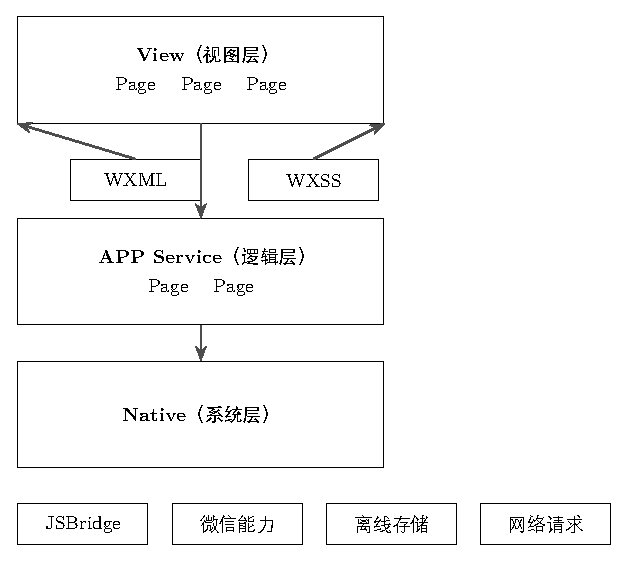
\includegraphics[width=0.72\textwidth]{figures/fig-architecture.pdf}
  \caption{刷题系统结构层次图}
  \label{fig:architecture}
\end{figure}

View（视图层）主要由 WXML、WXS 与 WXSS 组合编写，通过原生热布局的方式由组件来进行展示，主要用于将逻辑层的数据渲染到视图层，同时将视图层的事件传递给逻辑层。View 的 Component 以 Web Component 为标准，通过 Polymer 框架实现。Native 组件层在 Web View 层之上，由 View 的 Native Component 实现的组件有 \texttt{canvas}、\texttt{video}、\texttt{map}、\texttt{textarea} 等。

WXML（WeiXin Markup Language）是专门为微信小程序框架设计的标签语言，采用将基础组件和事件系统结合的方式构建页面的结构。WXML 类似于 HTML，是微信开发的一种标记语言，仅支持使用其指定的对应组件，例如 View、Block、Button、View-Scroll、Image、Text、Navigator 等。WXML 还具有数据绑定、列表渲染、条件渲染、模板、事件和引入等功能。其中，数据绑定使用双大括号进行双向绑定；列表渲染通过 \texttt{wx:for} 引用在 JavaScript 中定义的数组变量；条件渲染使用 \texttt{wx:if}、\texttt{wx:elif}、\texttt{wx:else} 判断。

WXS（WeiXin Script）是专门用于微信小程序的一套脚本语言，与 WXML 结合使用构建页面结构。WXS 能够在所有版本的微信小程序中运行，不依赖于当前运行的基础库版本。它拥有自己的语法规则，与 JavaScript 不一致，属于不同的编程语言。由于存在运行环境的差异，小程序内的 WXS 在 iOS 设备上运行会比 JavaScript 代码快 2 到 20 倍，在 Android 设备上二者运行效率相差无几。

WXSS（WeiXin Style Sheets）是专门为小程序设计的一套样式语言，用于描述页面结构中组件的显示方式，例如字体大小、背景颜色、定位方式等。为了便于前端开发者开发微信小程序，WXSS 具有 CSS 的大部分特性，并对 CSS 进行了扩充和修改\cite{bib:css,bib:html5}。与 CSS 相比，其扩展特性主要包括尺寸单位和样式导入两项。小程序使用 rpx（Responsive Pixel）作为尺寸单位，它是一个根据屏幕宽度自适应的尺寸单位，规定屏幕宽度为 750\,rpx。这意味着无论移动设备屏幕有多大，宽度都是 750 个 rpx；这是一个绝对大小，但是每个 rpx 的具体大小由移动终端的具体尺寸来决定。

APP Service（逻辑层）由 JavaScript 实现编写与封装，主要用于将逻辑层的数据进行处理后渲染到视图层，并对视图层用户行为的事件进行反馈。小程序各个页面中的网络通信、应用生命周期管理、数据管理以及页面路由都是由 App Service 实现的。由于页面是在 JsCore 中运行脚本逻辑，而 JsCore 是没有窗口对象的环境，所以小程序不能在脚本中使用 Document、Window 对象，也不能直接操作 DOM 节点和组件。因为 Zepto、jQuery 中使用了 Document、Window 等对象，所以它们在小程序中都无法被使用\cite{bib:jquery}。

Native（系统层）通过对微信客户端所提供的网络数据通信、文件系统管理、数据安全任务管理等基础功能进行封装，对上层提供一整套非常完整的 JavaScript API。由于小程序是通过 JSBridge 实现对底层原生 API 接口的调用，而 JSBridge 是架起上层开发与 Native（系统层）的桥梁，因此小程序可通过 API 直接使用原生的功能。

\subsection{微信小程序开发语言 JavaScript}

JavaScript 是一种通过解释执行的高级编程语言，是一门基于原型、函数先行、动态类型、面向对象的解释型语言。它已由 ECMA（欧洲电脑制造商协会）通过 ECMAScript 实现了语言的标准化。世界五大主流浏览器都已支持使用 JavaScript，绝大多数的网站都使用 JavaScript 实现动态交互\cite{bib:zakas}。JavaScript 支持面向对象编程、命令式编程以及函数式编程，它提供一系列的语法来控制节点、对象、日期、文本、数组以及正则表达式等。

一般情况下，完整的 JavaScript 包括以下几个部分：ECMAScript，用于描述该语言的语法和基本对象；文档对象模型（DOM），用于描述处理网页内容的方法和接口；浏览器对象模型（BOM），用于描述与浏览器进行交互的方法和接口。JavaScript 主要用于为 HTML 页面添加交互行为，可以直接嵌入 HTML 页面，单独引入的外部 JS 文件更有利于行为和结构的分离\cite{bib:ruan}。

与服务器端脚本语言不同，JavaScript 不需要服务器的支持，它被当作客户端的脚本语言在浏览器上运行。随着 HTML5、CSS3 语言标准的推行以及 JavaScript 事件驱动和异步 I/O 等特性的应用，它还可用于网络游戏、移动应用程序的开发以及在服务器端的网络环境运行，如 Node.js。

\subsection{微信 Web 开发工具}

微信 Web 开发者工具是由微信官方推出的专门用于帮助开发者更简单和高效地开发、调试微信小程序以及微信公众号的开发工具。它主要通过模拟微信客户端的表现，使开发者可以便捷地在 Mac 或者 PC 上进行开发和调试工作。它集成了小程序调试和公众号网页调试两种开发模式。使用小程序调试，开发者可以实现小程序的部分 API 的调用、代码查看和编辑、页面的开发调试、远程调试、小程序预览和发布等功能。

开发者可以直接在微信开发者工具中进行项目编辑、调试、预览、上传、编译、切换项目运行场景、模拟器尺寸以及切换模拟网络环境等。小程序在模拟器和真机上的运行效果基本相同，只是模拟器没有拨打电话、重力感应、发送短信、蓝牙等功能。但是由于运行环境的差异，部分 API 在开发者工具上的调试结果与真机的调试结果并不完全一致，例如 \texttt{wx.getUserInfo}、\texttt{wx.chooseInvoiceTitle} 等。因此，开发者如果需要进行调试，可以使用微信开发者工具的远程调试功能，并以真机调试为准。
